\documentclass[final,hyperref={pdfpagelabels=false}]{beamer}
\mode<presentation>
  {
  %  \usetheme{Berlin}
  \usetheme{Berlin}
  }
  \usepackage{times}
  \usepackage{amsmath,amsthm, amssymb, latexsym, amsfonts}
  %\boldmath
  \usepackage[english]{babel}
  \usepackage[latin1]{inputenc}
  \usepackage[orientation=landscape,size=a0,scale=1.4,debug]{beamerposter}

%\usepackage[dvips]{color}
\usepackage{graphics}
\usepackage{ulem}	%allows esoteric underlinings
\usepackage[all]{xy}	%xy-pic
\usepackage{bm}		%boldmath package - allows all math symbols to be boldened using \bm
\usepackage{wasysym}	%use for \apprge command
\usepackage{ifthen}
\usepackage{psfrag, psfig}
\usepackage{henon}


\theoremstyle{plain}%default
\newtheorem{mainthm}{Theorem}
\newtheorem{thm}{Theorem}
\newtheorem{lem}[thm]{Lemma}
\newtheorem{prop}[thm]{Proposition}
\newtheorem{cor}[thm]{Corollary}

\theoremstyle{definition}
\newtheorem{defn}[thm]{Definition}
\newtheorem{conj}[thm]{Conjecture}
\newtheorem*{cond}{Condition}
\newtheorem{ax}{Axiom}
\newtheorem{ass}{Assumptions}
\newtheorem*{claim}{Claim}

\theoremstyle{remark}
\newtheorem{rmk}[thm]{Remark}

%%%%%%%%%%%%%%%%%%%%%%%%%%%%%%%%%%%%%%%%%%%%%%%%%%%%%%%%%%%%%%%%%%%%%%%%%%%%%%%%%
\graphicspath{{figures/}}
\title[H\'enon Renormalisation]{H\'enon-like Maps and Renormalisation}
\author[Peter Hazard]{Peter Hazard}
\institute[IME-USP, S\~ao Paulo]{Instituto do Mathematics e \'Estatistica, Universidade de S\~ao Paulo}
\date{February 2010}

%%%%%%%%%%%%%%%%%%%%%%%%%%%%%%%%%%%%%%%%%%%%%%%%%%%%%%%%%%%%%%%%%%%%%%%%%%%%%%%%%
\begin{document}
\begin{frame}{}
\begin{columns}[t]
%%%%%%%%%%%%%%%%%%%%%%%%%%%%%%%%%%%%%%%%%%%%%%%%%%%%%%%%%%%%%%%%%%%%%%%%%%%%%%%%%
\begin{column}{0.3\linewidth}
\begin{block}{\maketitle}

We generalise the period doubling operator on the space of H\'enon-like maps introduced by de Carvalho, Lyubich and Martens to those of arbitrary stationary combinatorics.

\end{block}
\begin{block}{H\'enon-like Maps}
Let $\H_\Omega(\bar\e)$ denote the space H\'enon-like maps $F\in C^\omega(B,B)$ satisfying the following properties:
\begin{itemize}
\item $F$ is an orientation preserving diffeomorphism onto its image;
\item $F$ is expressible as
\begin{equation}
F(x,y)=(f(x)-\e(x,y),x)
\end{equation}
\item $f\colon J\to J$ is a real-analytic unimodal map 
\item $\e\colon B\to\RR$ is real-analytic and non-zero
\item $f$ and $\epsilon$ have holomorphic extensions to $\Omega_x$ and $\Omega$ respectively;
\item $\|\e\|_\Omega\leq \bar\e$. We call $\e$ an \emph{$\bar\e$-thickening}.
\end{itemize}
\vskip 20pt

Let $\U$ denote the space of unimodal maps on $J$. Let $\perm$ be a unimodal permutation on $W=\{0,1,\ldots, p-1\}$. 

\vskip 20pt

Then there exists a subspace $\U_\perm\subset\U$ on which the \emph{renormalisation operator} of type $\perm$, $\RU\colon \U_\perm\to\U$, is defined.

\vskip 25pt

\begin{thm}\label{R-construction}
For each $\perm$ there exist $C,\bar\e_0>0$ and a polydisk $\Omega\subset\CC$, such that: 
For any $\bar\e\in(0,\bar\e_0)$ there is a subspace $\H_{\Omega,\upsilon}(\bar\e)$ of $\H_{\Omega}(\bar\e)$ which contains $\U_\perm$ and an operator 
\[\RH\colon \H_{\Omega,\upsilon}(\bar\e)\to \H_{\Omega}(C\bar\e^p)\subset \H_{\Omega}(\bar\e)\]
which is a continuous extension of $\RU$.
\end{thm}
\end{block}
\begin{block}{The Renormalisation Operator}

More precisely, given $F(x,y)=(\phi(x,y),x)\in \H_{\Omega}(\bar\e)$ there is a map $H(x,y)$, called the \emph{horizontal diffeomorphism}, defined on a subdomain of $\Omega$. Then $F$ is \emph{pre-renormalisable} if $G=HF^pH^{-1}$ has an invariant square symmetric about the diagonal $\{x=y\}$.
Define the \emph{renormalisation of $F$} by 
\begin{equation}
\RH F=IGI^{-1}=IHF^pH^{-1}I^{-1}=\MT^{-1} F^p\MT
\end{equation}
where $I$ is a suitable affine map and $\MT=H^{-1}\circ I^{-1}$ is a non-affine map called the \emph{Scope Map}.
\vskip 20pt
It is know that the unimodal renormalisation operator $\RU$ has a unique hyperbolic fixed point $f_*$ with codim.-one stable manifold.
\vskip 5pt
\end{block}
\end{column}



%%%%%%%%%%%%%%%%%%%%%%%%%%%%%%%%%%%%%%%%%%%%%%%%%%%%%%%%%%%%
\begin{column}{0.3\linewidth}
\begin{block}{The Renormalisation Operator ctd.}
\begin{figure}[htp]
\centering
\tiny
\psfrag{j0}{$\oo{0}{J}$}
\psfrag{j1}{$\oo{1}{J}$}
\psfrag{j2}{$\oo{2}{J}$}
\psfrag{b0}{$\oo{0}{B}$}
\psfrag{b1}{$\oo{1}{B}$}
\psfrag{b2}{$\oo{2}{B}$}
\psfrag{b0diag}{$\oo{0}{B}_\diag$}
\psfrag{b1diag}{$\oo{1}{B}_\diag$}
\psfrag{b2diag}{$\oo{2}{B}_\diag$}
\psfrag{H}{$H$}
\psfrag{Hi}{$\bar H$}

\psfrag{I}{$I$}
\psfrag{line0}{$Im(F) \ \mbox{or} \ Im(\RH F)$}
\psfrag{line1}{$Im(G)$}
\psfrag{line2}{the strip $S$}
\psfrag{line3}{the renormalisation cycle}

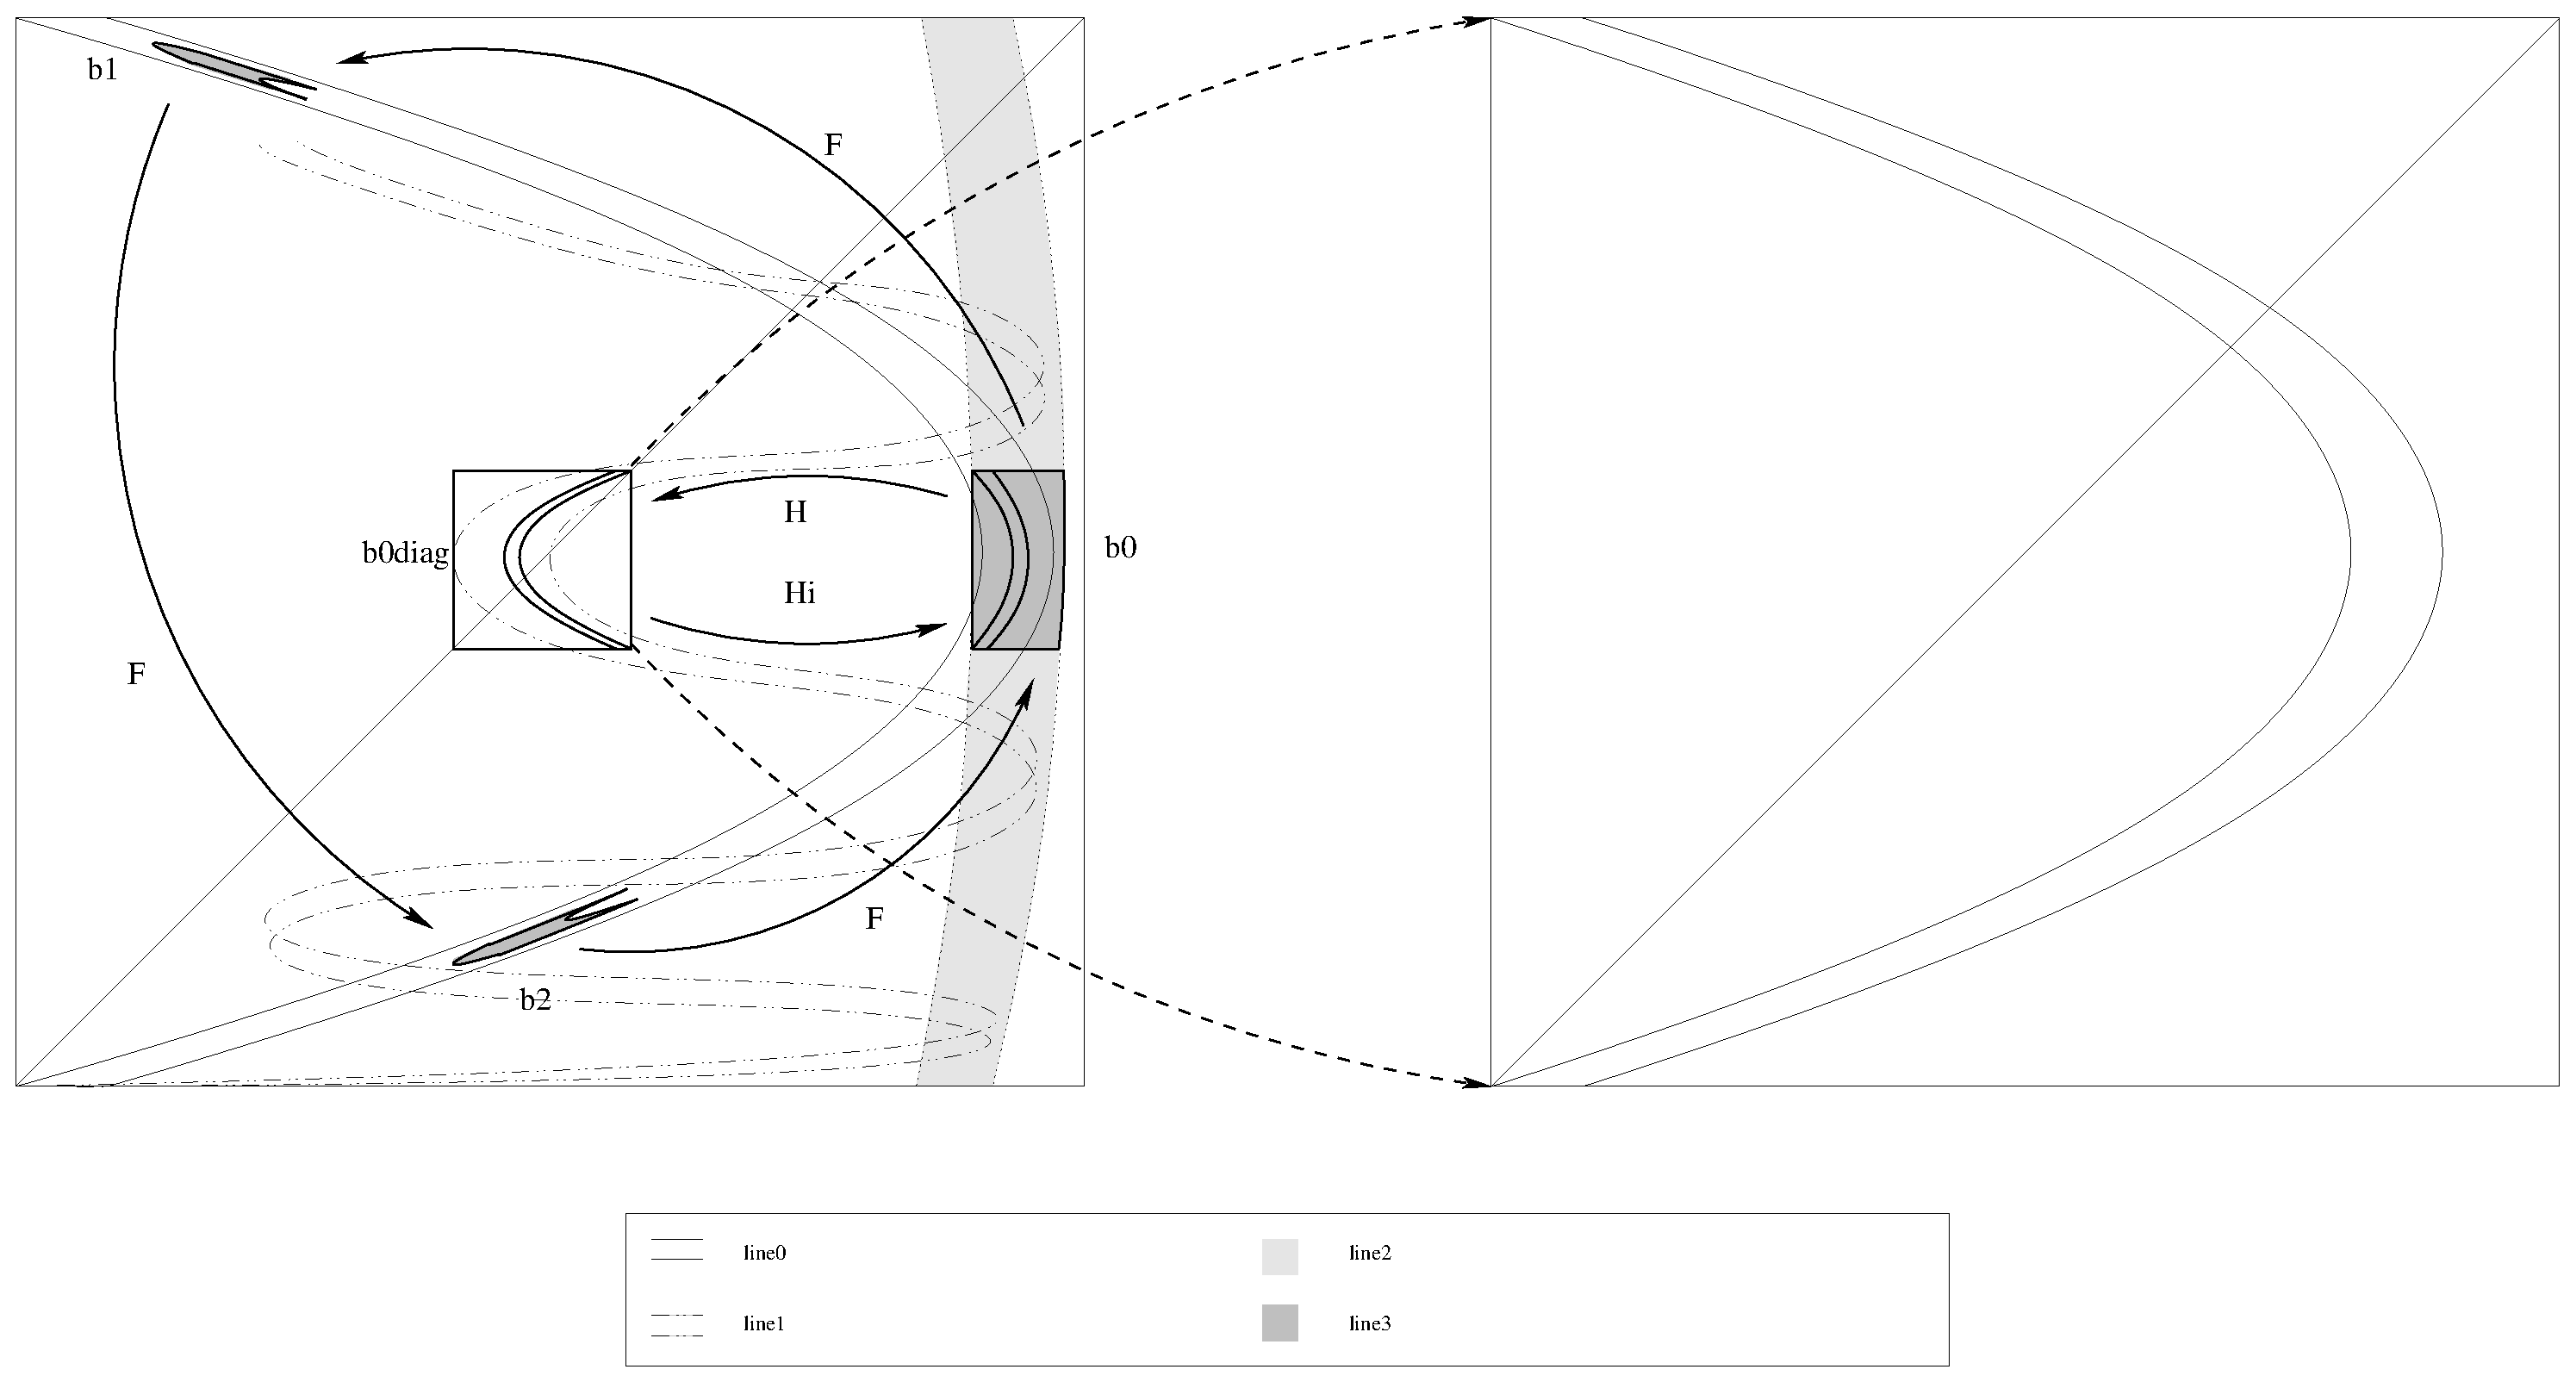
\includegraphics[scale=0.65]{period3-henon-5.eps}
\vspace*{0.1cm}
\caption{A renormalisable H\'enon-like map whose combinatorial type is period tripling. Here the dashed lines represent the image of the square $B$ under the pre-renormalisation $G$.}\label{fig:renorm-henon}
\end{figure}
\begin{thm}\label{R-convergence}
For each $\perm$ there exists a $\bar\e_0>0$ such that for all $0<\bar\e<\bar\e_0$ 
\begin{itemize}
\item the operator
$\RH\colon \H_{\Omega,\upsilon}(\bar\e)\to\H_{\Omega}(\bar\e)$
has a unique fixed point $F_*=(f_*,\pi_x)$ where $f_*$ is the fixed point of $\RU$;
\item $F_*$ is hyperbolic and has a codimension-one stable manifold.
\end{itemize}
\end{thm}
\end{block}


\begin{block}{Infinitely Renormalisable Maps}
Let $\I_{\Omega,\perm}(\bar\e)\subset \H_{\Omega}(\bar\e)$ denote the space of infinitely renormalisable maps.
Let  
\begin{itemize}
\item $W^n$ denote the set of words $\word{w}{}$ of length $n$, 
\item $W^*$ denote the set of words $\word{w}{}$ of arbitrary finite length,
\item $\bar W$ denote the set of words $\word{w}{}$ of infinite length.
\end{itemize}
We endow both $W^*$ and $\bar W$ with the structure of a $p$-adic adding machine, denoted by $\word{w}{}\mapsto 1+\word{w}{}$.

\begin{figure}[tp]
\centering
\tiny
\psfrag{...}{$\cdots$}

\psfrag{a}{$0$}
\psfrag{amt}{$\oo{0}{\MT_0}$}
\psfrag{ab0}{$\oo{0}{B_0}$}
\psfrag{ab1}{$\oo{1}{B_0}$}
\psfrag{ab2}{$\oo{2}{B_0}$}
\psfrag{af0}{$F_0$}
\psfrag{af1}{$F_0$}
\psfrag{af2}{$F_0$}


\psfrag{b}{$1$}
\psfrag{bmt}{$\oo{0}{\MT_1}$}
\psfrag{bb0}{$\oo{0}{B_1}$}
\psfrag{bb1}{$\oo{1}{B_1}$}
\psfrag{bb2}{$\oo{2}{B_1}$}
\psfrag{bf0}{$F_1$}
\psfrag{bf1}{$F_1$}
\psfrag{bf2}{$F_1$}

\psfrag{c}{$2$}
\psfrag{cmt}{$\oo{0}{\MT_2}$}
\psfrag{cb0}{$\oo{0}{B_2}$}
\psfrag{cb1}{$\oo{1}{B_2}$}
\psfrag{cb2}{$\oo{2}{B_2}$}
\psfrag{cf0}{$F_2$}
\psfrag{cf1}{$F_2$}
\psfrag{cf2}{$F_2$}

%\reflectbox
\vspace*{0.2cm}
\caption{Scope maps for a period-3 infinitely renormalisable H\'enon-like map.}\label{fig:scopemaps-henon}
\end{figure}

For $F\in \I_\Omega(\bar\e)$ let  $F_n=\RH^n F$. Let $\MT_n=\MT(F_n)$ be called the \emph{Scope Map of height $n$}.
For $w\in W$, $\word{w}{}=w_0\ldots w_{m-1}\in W^m$ let
\begin{itemize}
\item $\MT_n^w=\o{w}{F_n}\circ \MT_n$;
\item $\MT_n^{\word{w}{}}=\MT_{n}^{w_0}\circ\cdots\circ\MT_{n+m}^{w_{m-1}}$;
\item $B_n^{\word{w}{}}=\MT_n^{\word{w}{}}(B)$.
\end{itemize}
The maps $\MT_n^{\word{w}{}}$ are called the \emph{$\word{w}{}$-Scope Maps at height $n$}. The $B_n^{\word{w}{}}$ are called the \emph{canonical boxes of height $n$} and the collection $\uline{B}$ of all canonical boxes is called the \emph{canonical boxing}. 
\end{block}

\end{column}
%%%%%%%%%%%%%%%%%%%%%%%%%%%%%%%%%%%%%%%%%%%%%%%%%%%%%%%%%%%%%%%%%%%%%%%%
\begin{column}{0.3\linewidth}
\begin{block}{Universality, Non-Rigidity and Unbounded Geometry}
\begin{thm}[Invariant Cantor Set]
Let $F\in\I_{\Omega}(\bar\e)$. Then there exists an $F$-invariant Cantor set $\Cantor\subset B$ upon which $F$ acts as the $p$-adic adding machine.  Moreover, there exists a unique $F$-invariant measure $\mu$ whose support is the Cantor set $\Cantor$.
\end{thm}
For an $F\in\I_{\Omega,\perm}(\e)$ we now define the \emph{Average Jacobian} to be
\begin{equation}
b(F)=\exp\int\log \jac{F}{z} d\mu(z)
\end{equation}
For the H\'enon maps $F(x,y)=(a-x^2-by,x)$ this is just $b$.

\vskip 10pt

\begin{thm}[Universality]
Let $F\in\I_{\Omega,\perm}(\bar\e)$. Then
\begin{equation}
F_n(x,y)=(f_n(x)-a(x)yb^{p^n}(1+\bigo(\rho^n)),x)
\end{equation}
\vspace{0.15in}
where $b$ is the average Jacobian of $F$, $f_n\in\U$ and $f_n\to f_*$ exponentially and $a\in C^\omega(I,\RR)$ and $0<\rho<1$ are universal.
\end{thm}
This universal limiting behaviour also occurs in the unimodal theory.
However, in contrast, we get the following.

\vskip 10pt

\begin{thm}[Non-Rigidity]
Let $F_0, F_1\in \I_{\Omega}(\bar\e)$ be two infinitely renormalisable H\'enon-like maps. Let us denote 
\begin{itemize}
\item their respective average Jacobians by $b_0, b_1$; 
\item their respective Cantor sets by $\Cantor_0, \Cantor_1$.
\end{itemize}
Then  any conjugation $\Gamma\colon \Cantor_0\to\Cantor_1$ sending $\tau_0$ to $\tau_1$ is at most $C^{\alpha}$ where
\begin{equation}
\alpha\leq \frac{1}{2}\left(1+\frac{\log b_0}{\log b_1}\right)
\end{equation}
\end{thm}
The boxing $\uline{B}=\{B^{\word{w}{}}\}_{\word{w}{}\in W_p^*}$ has \emph{bounded geometry} if there exist constants $0<\kappa<1<C$, such that for all $\word{w}{}\in W_p^*$ and
$w,\tilde{w}\in W_p$,
\begin{align*}
C^{-1}\dist(B^{\word{w}{w}},B^{\word{w}{\tilde{w}}})
<\diam(B^{\word{w}{w}})<
C\dist(B^{\word{w}{w}},B^{\word{w}{\tilde{w}}}), \\
 \notag \\
\kappa\diam(B^{\word{w}{}})<\diam(B^{\word{w}{w}})<(1-\kappa)\diam(B^{\word{w}{}}).
\end{align*}
We will say that $\Cantor$ has \emph{bounded geometry} if there exists a boxing $B^{\word{w}{}}$ of $\Cantor$ with bounded geometry. Otherwise $\Cantor$ has \emph{unbounded geometry}.

\vskip 10pt

\begin{thm}[Generic Unbounded Geometry]
Given a one-parameter family $F_b\in\I_{\Omega}(\bar\e)$ such that $b(F_b)=b$ there exists $b_0>0$ and $S\subset (0,b_0]$, a dense $G_\delta$ set with full (relative) Lebesgue measure such that $F_b$ has unbounded geometry whenever $b\in S$.
\end{thm}

\end{block}
\end{column}
\end{columns}
\end{frame}

\end{document}



%%%%%%%%%%%%%%%%%%%%%%%%%%%%%%%%%%%%%%%%%%%%%%%%%%%%%%%%%%%%%%%%%%%%%%%%%%%%%%%%%%%%%%%%%%%%%%%%%%%%
%%% Local Variables: 
%%% mode: latex
%%% TeX-PDF-mode: t
%%% End:
